\documentclass[%
reprint,
amsmath,
amssymb,
aps,
]{revtex4-1}

\usepackage{graphicx}
\usepackage[mathletters]{ucs} % Extended unicode (utf-8) support
\usepackage[utf8x]{inputenc}
\usepackage{hyperref}
\usepackage{mhchem}


\begin{document}


\title{Perhitungan struktur elektronik berdasarkan teori fungsional
    kerapatan dengan fungsi basis Lagrange: Implementasi awal}
\author{Fadjar Fathurrahman}
\affiliation{Pusat Penelitian Nanosains dan Nanoteknologi, Institut Teknologi Bandung}

\begin{abstract}
This is the abstract.
\end{abstract}

\maketitle

\section{Pendahuluan}

Peran komputasi dalam nanosains dan nanoteknologi.

Teori fungsional kerapatan (\emph{density functional theory}).

Peran teori fungsional kerapatan

\section{Teori}

Berdasarkan teori fungsional kerapatan,
energi total dari sistem yang terdiri dari elektron yang berinteraksi
dengan suatu potential eksternal $V_{\mathrm{ext}}(\mathbf{r})$
dapat dinyatakan sebagai
\begin{widetext}
\begin{equation}
E[\rho(\mathbf{r})] = 
-\frac{1}{2}\sum_{i}f_{i}
\int\mathrm{d}\mathbf{r}\,
\, \psi^{*}_{i}(\mathbf{r}) \nabla^2 \psi_{i}(\mathbf{r})
+ \int\mathrm{d}\mathbf{r}\,
\rho(\mathbf{r}) V_{\mathrm{ext}}(\mathbf{r})
+
\frac{1}{2}\int\mathrm{d}\mathbf{r}\,\mathrm{d}\mathbf{r}'\,
\frac{\rho(\mathbf{r})\rho(\mathbf{r}')}{\left|\mathbf{r}-\mathbf{r}'\right|}
+ E_{\mathrm{xc}}[\rho(\mathbf{r})]
\end{equation}
\end{widetext}

LDA XC:
\begin{equation}
E_{\mathrm{xc}}[\rho(\mathbf{r})] =
\int\mathrm{d}\mathbf{r}\,
\varepsilon_{\mathrm{xc}}(\rho(\mathbf{r}))
\rho(\mathbf{r})
\end{equation}

\begin{equation}
V_{\mathrm{xc}}(\mathbf{r}) = \varepsilon_{\mathrm{xc}}(\rho(\mathbf{r}))
+ \rho(\mathbf{r})\frac{\mathrm{d}\varepsilon_{\mathrm{xc}}(\rho)}{\mathrm{d}\rho}
\end{equation}

Persamaan sentral pada teori fungsional kerapatan adalah persamaan
Kohn-Sham yang dapat ditulis sebagai berikut.
\begin{equation}
\left[
-\frac{1}{2}\nabla^2
+ V_{\mathrm{Ha}}(\mathbf{r})
+ V_{\mathrm{xc}}(\mathbf{r})
+ V_{\mathrm{ext}}(\mathbf{r})
\right]\psi_{i}(\mathrm{r}) =
\epsilon_{i} \psi_{i}(\mathrm{r})
\label{eq:KS_eq}
\end{equation}
Suku potensial pertama pada persamaan $\eqref{eq:KS_eq}$,
$V_{\mathrm{Ha}}(\mathbf{r})$ menyatakan potensial Hartree,
\begin{equation}
V_{\mathrm{Ha}}(\mathbf{r}) =
\int
\frac{\rho(\mathbf{r}')}{\left|\mathbf{r} - \mathbf{r}'\right|}
\mathrm{d}\mathbf{r}'
\end{equation}
dengan $\rho(\mathbf{r})$ adalah kerapatan (muatan) elektron
yang dapat ditulis sebagai
\begin{equation}
\rho(\mathbf{r}) = \sum_{i} f_{i}\, \psi^{*}_{i}(\mathbf{r}) \psi_{i}(\mathbf{r})
\end{equation}
Suku potensial ketida adalah $V_{\mathrm{ext}}(\mathbf{r})$
yang menyatakan potensial eksternal yang dirasakan oleh elektron.


\section{Fungsi basis Lagrange}

Untuk suatu interval $[0,L_{\alpha}]$ yang diberikan, dengan $L_{\alpha} > 0$, titik grid
$x_{\alpha}$ sesuai untuk fungsi basis
Lagrange periodik dapat dinyatakan dengan persamaan berikut.
\begin{equation}
x_{\alpha} = \frac{L_{\alpha}}{2}\frac{2\alpha-1}{N_{a}}
\end{equation}
Fungsi basis Lagrange periodik yang akan digunakan
memiliki bentuk sebagai berikut.
\begin{equation}
\phi_{\alpha}(x) = \frac{1}{\sqrt{N_{\alpha}L_{\alpha}}}
\sum_{n_{\alpha}=1}^{N_{\alpha}} \cos\left[
\frac{\pi}{L_{\alpha}}(2n_{\alpha} - N_{\alpha} - 1)(x-x_{\alpha})
\right]
\end{equation}

Test
\begin{figure}
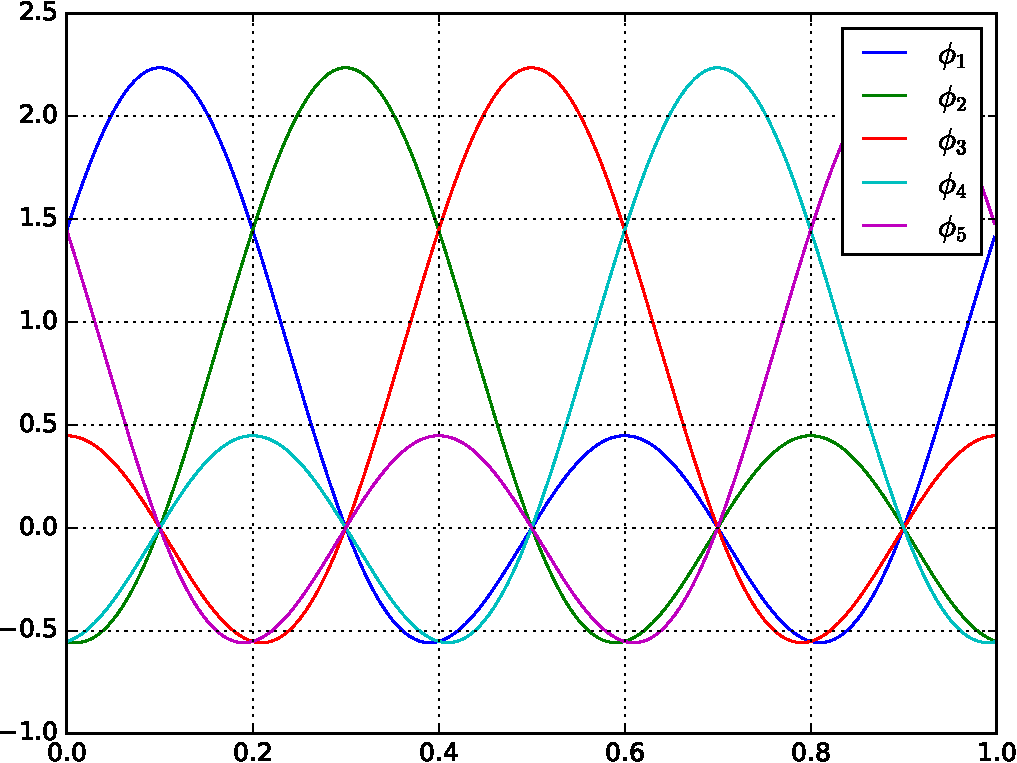
\includegraphics[scale=0.5]{images/plotN_5.pdf}
\end{figure}

Sembarang fungsi periodic $f(x) = f(x+L_{\alpha})$ dapat diekspansi dalam fungsi basis
Lagrange
\begin{equation}
f(x) = \sum_{\alpha}^{N_{\alpha}} c_{\alpha} \phi_{\alpha}(x)
\end{equation}
dengan $c_{\alpha}$ adalah koefisien ekspansi.
Nilai fungsi $f(x)$ pada titik grid $x_{\alpha}$ dapat diperoleh langsung
dari koefisien ekspansi melalui hubungan
$c_{\alpha} = \sqrt{L_{\alpha}/N_{\alpha}}f(x_{\alpha})$.

Ekspansi persamaan Kohn-Sham dengan fungsi basis Lagrange:
\begin{equation}
\psi_{i}(\mathbf{r}) = \sum_{\alpha\beta\gamma}
C^{i}_{\alpha\beta\gamma} \Phi_{\alpha\beta\gamma}(\mathbf{r})
\end{equation}
dengan fungsi basis \cite{Baye2015}
\begin{equation}
\Phi_{\alpha\beta\gamma}(\mathbf{r}) =
\phi_{\alpha}(x)\phi_{\beta}(y)\phi_{\gamma}(z)
\end{equation}




\section{Perhitungan}

Potensial eksternal berupa fungsi Gaussian:
\begin{equation}
V_{\mathrm{ext}}(r) = A\exp(-\alpha r^2)
\end{equation}

Menggunakan bagian lokal dari pseudopotensial HGH

Contoh molekul diatomik: $\ce{H2}$ dan LiH

Visualisasi orbital molekul

\section{Kesimpulan}

Implementasi

\bibliography{LFDFT-v1}

\end{document}
